\section{From double categories to bicategories}
\label{sec:1x1-to-bicat}

We are now equipped to lift structures on double categories to
their loose bicategories.  In this section we show that passage
from double categories to bicategories is given by a functor of locally cubical bicategories. In order to prove this, we first give an intermediate result that $\cH$ lifts to a functor of hom-bicategories
\begin{align}
    \cDbl(\lD,\lE) &\too \cBicat(\cH(\lD),\cH(\lE))
\end{align}

As a point of notation, we write $\odot$ for the composition of
1-cells in a bicategory, since our bicategories are generally of the
form $\cH(\lD)$.  As advocated by Max Kelly, we say \textbf{functor}
to mean a morphism between bicategories that preserves composition up
to coherent isomorphism; equivalent terms include \emph{weak 2-functor},
\emph{pseudofunctor}, and \emph{homomorphism}.
We will not discuss lax functors (a.k.a. ``morphisms'') between bicategories at all in this paper.

Recall that the assignment $\cH$ sends each double category $\lC$ to the loose bicategory  $\cH(\lD)$ of objects, 1-cells, and globular 2-morphisms of $\lD$.  Note that functors of double categories and bicategories compose strictly associatively; hence, we can talk about the 1-categories of double categories and bicategories, which we denote ${\bf Dbl}$ and ${\bf Bicat}$ respectively.

\begin{thm}\label{thm:1-func}
 If \lD\ is a double category, then $\cH(\lD)$ is a bicategory, and
  any functor $F\maps \lD\to\lE$ induces a functor $\cH(F)\maps
  \cH(\lD)\to\cH(\lE)$.  In this way $\cH$ defines a functor of
  1-categories $\mathbf{Dbl}\to \mathbf{Bicat}$.
\end{thm}
\begin{proof}
 The constraints of $F$ are all globular, hence give constraints for
  $\cH(F)$.  Functoriality is evident.
\end{proof}

% MS: This doesn't really make precise sense, and I'm not sure it's necessary.
%Note that this is a stronger condition than we need for our main result.
The action of \cH\ on transformations is less obvious. It
requires the presence of companions or conjoints to lift the part of the data given by vertical morphisms to loose 1-cells. Before we discuss how this works, we briefly recall some definitions regarding transformations between functors of bicategories.

If $F,G\maps \cA\to\cB$ are functors between bicategories, then an
\textbf{oplax transformation} $\al\maps F\to G$ consists of 1-cells
$\al_A\maps FA\to GA$ and 2-cells
\[\vcenter{\xymatrix{ \ar[r]^{Ff}\ar[d]_{\al_A} \drtwocell\omit{\al_f} &  \ar[d]^{\al_B}\\
  \ar[r]_{Gf} & }}\]
such that for any 2-cell $\xymatrix{A \rtwocell^f_g{x} & B}$ in \cA,
\begin{equation}
  \label{eq:laxtransf-nat}
  \vcenter{\xymatrix@R=1pc@C=3pc{
      \rtwocell^{Ff}_{Fg}{Fx}\ar[dd]_{\al_A} 
      &  \ar[dd]^{\al_B}\\
      \drtwocell\omit{\al_g} & \\
      \ar[r]_{Gg} & }}\;=\;
  \vcenter{\xymatrix@R=1pc@C=3pc{
      \ar[r]^{Ff}\ar[dd]_{\al_A} \drtwocell\omit{\al_f} &
      \ar[dd]^{\al_B}\\ & \\
      \rtwocell^{Gf}_{Gg}{Gx} & }}
\end{equation}
and moreover for any $A$ and any $f,g$ in \cA,
\begin{equation}
  \vcenter{\xymatrix@R=5pc{
      \rtwocell^{1_{FA}}_{F(1_A)}{\iso} \ar[d]_{\al_A} \drtwocell\omit{\al_{1_A}} &  \ar[d]^{\al_A}\\
      \rtwocell^{G(1_A)}_{1_{GA}}{\iso} & }} \;=\;
  \vcenter{\xymatrix{ \ar[r]^{1_{FA}}\ar[d]_{\al_A} \drtwocell\omit{\iso}&  \ar[d]^{\al_A}\\
      \ar[r]_{1_{GA}} &
    }}
  \quad\text{and}\quad
  \vcenter{\xymatrix{
      \ar[r]|{Ff}\ar[d]_{\al_A} \drtwocell\omit{\al_f}
      \rruppertwocell^{F(gf)}{\iso}
      &
      \ar[r]|{Fg}\ar[d]|{\al_B} \drtwocell\omit{\al_g} &
      \ar[d]^{\al_C}\\
      \ar[r]|{Gf} \rrlowertwocell_{G(gf)}{\iso} & \ar[r]|{Gg} & }}
  \;=\;
  \vcenter{\xymatrix{ \ar[r]^{F(gf)}\ar[d]_{\al_A} \drtwocell\omit{\al_{gf}} &  \ar[d]^{\al_C}\\
      \ar[r]_{G(gf)} & }}\label{eq:laxtransf-ax}
\end{equation}
It is a \textbf{lax transformation} if the 2-cells $\al_f$ go the
other direction, and a \textbf{pseudo transformation} if they are
isomorphisms.

When two functors of bicategories agree on objects, there is a simpler notion of transformation between them, called an \emph{icon}.
An icon is, morally speaking, an oplax transformation whose 1-cell components are all identities; but as noted by~\cite{lack:icons} this can be reexpressed without referring to these identity morphisms at all, yielding a definition that is easier to work with (because identity 1-cells in a bicategory are not strict).

\begin{defn}
Let $\cD, \cE$ be bicategories, and let $F,G: \cD \rightarrow \cE$ be functors that agree on objects. An \textbf{icon} $\alpha: F \Rightarrow G$ is given by a family of 2-cells $\alpha_f : Ff \Rightarrow Gf$ indexed by the 1-cells of $\cD$, which are natural in $f$ and such that for all objects $A, B, C$ and 1-cells $A \xrightarrow{f} B \xrightarrow{g} C$ the following equations hold:
%\[
%\begin{tikzpicture}[yscale=1,xscale=1.5]
%\node (tl) at (0,1) {$I_{FA}$};
%\node (tr) at (1,1) {$F I_A$};
%\node (bl) at (0,0) {$I_{GA}$};
%\node (br) at (1,0) {$GI_A$};
%\draw[->] (tl) to node[above]{$\phi$} (tr);
%\draw[->] (bl) to node[below]{$\phi$} (br);
%\draw[doubleeq] (tl) to (bl);
%\draw[->] (tr) to node[right]{$\alpha_{I_A}$} (br);
%\end{tikzpicture}
%\qquad
%\begin{tikzpicture}[yscale=1, xscale=1.5]
%\node (tl) at (0,1) {$F(g)  F(f)$};
%\node (tr) at (1,1) {$F(g  f)$};
%\node (bl) at (0,0) {$G(g)  G(f)$};
%\node (br) at (1,0) {$G(g  f)$};
%\draw[->] (tl) to node[above]{$\phi$} (tr);
%\draw[->] (bl) to node[below]{$\phi$} (br);
%\draw[->] (tl) to node[left]{$\alpha_g \tens \alpha_f$}(bl);
%\draw[->] (tr) to node[right]{$\alpha_{g \tens f}$} (br);
%\end{tikzpicture}
%\]

\begin{equation}\label{eq:iconeq}
\begin{aligned}
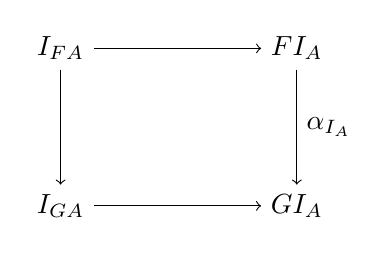
\begin{tikzpicture}[yscale=2,xscale=3]
\node (tl) at (0,1) {$I_{FA}$};
\node (tr) at (1,1) {$F I_A$};
\node (bl) at (0,0) {$I_{GA}$};
\node (br) at (1,0) {$GI_A$};
\draw[->] (tl) to node[above]{$\iso$} (tr);
\draw[->] (bl) to node[below]{$\iso$} (br);
\draw[->] (tl) to node[left]{$\iso$} (bl);
\draw[->] (tr) to node[right]{$\alpha_{I_A}$} (br);
\end{tikzpicture}
\end{aligned}
\qquad
\begin{aligned}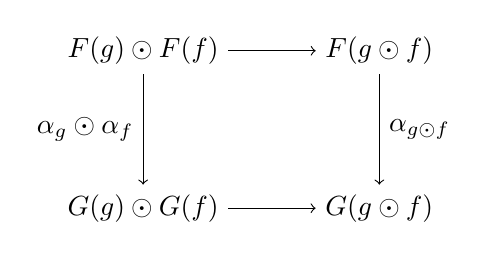
\begin{tikzpicture}[yscale=2, xscale=3]
\node (tl) at (0,1) {$F(g) \odot F(f)$};
\node (tr) at (1,1) {$F(g \odot f)$};
\node (bl) at (0,0) {$G(g) \odot G(f)$};
\node (br) at (1,0) {$G(g \odot f)$};
\draw[->] (tl) to node[above]{$\iso$} (tr);
\draw[->] (bl) to node[below]{$\iso$} (br);
\draw[->] (tl) to node[left]{$\alpha_g \odot \alpha_f$}(bl);
\draw[->] (tr) to node[right]{$\alpha_{g \odot f}$} (br);
\end{tikzpicture}
\end{aligned}
\end{equation}
\end{defn}


Recall also that if $\al,\al'\maps F\to G$ are oplax transformations,
a \textbf{modification} $\mu\maps \al\to\al'$ consists of 2-cells
$\mu_A\maps \al_A\to\al'_A$ such that
\begin{equation}
  \vcenter{\xymatrix@C=1pc@R=2.5pc{ \ar[rr]^{Ff}\dtwocell_{\al'_A}^{\al_A}{\mu_A}  &
      \drtwocell\omit{\al_f} &  \ar[d]^{\al_B}\\
      \ar[rr]_{Gf} && }} \quad=\quad
  \vcenter{\xymatrix@C=1pc@R=2.5pc{ \ar[rr]^{Ff}\ar[d]_{\al'_A} \drtwocell\omit{\al'_f} && 
      \dtwocell^{\al_B}_{\al'_B}{\mu_B}\\
      \ar[rr]_{Gf} && }}\label{eq:modif-ax}
\end{equation}
There is an evident notion of modification between lax transformations
as well.
We have three bicategories
\[ \cBicat_c(\cA,\cB) \qquad \cBicat_l(\cA,\cB) \qquad \cBicat_p(\cA,\cB) \]
whose objects are the functors $\cA\to\cB$, whose morphisms are colax, lax, and pseudo transformations respectively, and whose 2-morphisms are modifications.

A \textbf{pseudo natural adjoint equivalence} is, by definition, an internal adjoint equivalence in $\cBicat_p(\cA,\cB)$.
However, by doctrinal adjunction~\cite{kelly:doc-adjn}, an internal adjoint equivalence in $\cBicat_c(\cA,\cB)$ or $\cBicat_l(\cA,\cB)$ is automatically pseudo natural as well.

Let $\cDblcf$ denote the sub-2-category of $\cDbl$ containing all double categories and all functors between them, but only the tight transformations $\al:F\to G: \lD\to\lE$ such that each tight component $\al_A$ has a loose companion $\widehat{\al_A}$.
Note that if \lE\ is isofibrant, every invertible $\al$ has this property, and if \lE\ has companions for all tight 1-morphisms then every transformation has this property.

\begin{thm}\label{thm:h-locfr}
  We have a functor of bicategories
  \begin{align}
    \cDblcf(\lD,\lE) &\too \cBicat_c(\cH(\lD),\cH(\lE))\\
    F &\mapsto \cH(F)\\
    \al &\mapsto \alhat.
  \end{align}
\end{thm}

Note that we are here regarding the 1-category $\cDblcf(\lD,\lE)$ as a bicategory with only identity 2-cells.
Since any functor of bicategories preserves adjoint equivalences, and an adjoint equivalence in a mere category is simply an isomorphism, it follows that if $\al$ is an isomorphism then $\alhat$ is (equipped with the structure of) a pseudo natural adjoint equivalence.

\begin{proof}
  We define the 1-cell components of $\alhat$ by choosing companions $\alhat_A = \widehat{\al_A}$ of each component of $\al$.
  The 2-cell component $\alhat_f$ is the composite
  \begin{equation}
    \vcenter{\xymatrix@R=1.5pc@C=2.5pc{
        \ar[r]|-@{|}^{U_{FA}}\ar@{=}[d] \ar@{}[dr]|{\Downarrow \eta_{\hat{\alpha}_A}} &
        \ar[r]^{Ff}\ar[d]|{\al_A} \ar@{}[dr]|{\Downarrow \al_f} &
        \ar[r]|-@{|}^{\alhat_B}\ar[d]|{\al_B} \ar@{}[dr]|{\Downarrow \epsilon_{\hat{\alpha}_B}} &
        \ar@{=}[d]\\
        \ar[r]|-@{|}_{\alhat_A} &
        \ar[r]_{Gf} &
        \ar[r]|-@{|}_{U_{GB}} & 
      }}\label{eq:oplax-2cell}
%     \vcenter{\xymatrix@R=1.5pc@C=2.5pc{
%         \ar[r]|-@{|}^{Ff}\ar@{=}[d] \ar@{}[drrr]|{\iso} &
%         \ar[rr]|-@{|}^{\alhat_B} &&
%         \ar@{=}[d]\\
%         \ar[r]|-@{|}^{U_{FA}}\ar@{=}[d] \ar@{}[dr]|{\Downarrow} &
%         \ar[r]|{Ff}\ar[d]|{\al_A} \ar@{}[dr]|{\Downarrow \al_f} &
%         \ar[r]|-@{|}^{\alhat_B}\ar[d]|{\al_B} \ar@{}[dr]|{\Downarrow} &
%         \ar@{=}[d]\\
%         \ar[r]|-@{|}_{\alhat_A} \ar@{=}[d] \ar@{}[drrr]|\iso &
%         \ar[r]|{Gf} &
%         \ar[r]|-@{|}_{U_{GB}} & \ar@{=}[d]\\
%         \ar[r]|-@{|}_{\alhat_A} & \ar[rr]|-@{|}_{Gf} &&
%       }}\label{eq:oplax-2cell}
  \end{equation}
  Equations~\eqref{eq:laxtransf-nat} and~\eqref{eq:laxtransf-ax}
  follow directly from \autoref{thm:dbl-transf}.

  It is left to construct the constraints and check the axioms for functors of bicategories. Suppose we are given $\al\maps F\to G$ and $\be\maps G\to H$.  Then by
  \autoref{thm:comp-compose}, $\behat_A\odot\alhat_A$ is a companion
  of $\be_A\circ \al_A$, so we have a canonical isomorphism given by the icon
  \[\theta_{\widehat{\be\al}_A, \,\behat_A\odot\alhat_A}\maps
  \widehat{\be\al}_A \too[\iso] \behat_A\odot\alhat_A.
  \]
  Of course, we also have $\theta_{\widehat{1_A},U_A}\maps
  \widehat{1_A} \too[\iso] U_A$ by \autoref{thm:comp-unit}.  These
  constraints are automatically natural, since $\cDbl(\lD,\lE)$ has no
  nonidentity 2-cells.  The axiom for the composition constraint says
  that two constructed isomorphisms of the form
  \[\widehat{\gm\be\al}_A \too[\iso] (\gmhat_A \odot \behat_A)\odot \alhat_A\]
  are equal.  However, both $\widehat{\gm\be\al}_A$ and $(\gmhat_A
  \odot \behat_A)\odot \alhat_A$ are companions of $\gm_A\be_A\al_A$,
  and both of these isomorphisms are constructed from composites of $\theta$s;
  hence they are both equal to
  \[\theta_{\widehat{\gm\be\al}_A,\, (\gmhat_A \odot \behat_A)\odot
    \alhat_A}\] and thus equal to each other.  The same argument
  applies to the axioms for the unit constraint; thus we have a functor of bicategories.
\end{proof}

Of course, the functor constructed in \cref{thm:h-locfr} depends on the choices of companions made in the proof.
However up to equivalence it does not depend on these choices:

\begin{lem}\label{thm:h-locfr-uniq}
  Suppose we make two different sets of choices of companions for each component of a tight transformation in $\cDblcf(\lD,\lE)$, yielding by the proof of \cref{thm:h-locfr} two different functors
  \[\cH,\cH'\maps \cDblcf(\lD,\lE)\too \cBicat_c(\cH(\lD),\cH(\lE)).\]
  Then the isomorphisms $\theta$ from \autoref{thm:theta} fit together
  into an invertible icon $\cH\cong \cH'$.
\end{lem}
\begin{proof}
  We must first show that for a given transformation $\al\maps F\to
  G\maps \lD\to\lE$ in \cDbl, the isomorphisms \th\ correspond to 2-cells $\alhat \iso \alhat'$ of $\cBicat_c(\cH(\lD),\cH(\lE))$; that is, they form invertible
  modifications.
  Substituting~\eqref{eq:oplax-2cell} and the definition of \th\
  into~\eqref{eq:modif-ax}, this becomes the assertion that
  \begin{equation}
    \vcenter{\xymatrix@R=1.5pc@C=2pc{
        &
        \ar[r]|-@{|}^{U_{FA}}\ar@{=}[d] \ar@{}[dr]|{\Downarrow \eta_{\hat{\alpha}_A}} &
        \ar[r]^{Ff}\ar[d]|{\al_A} \ar@{}[dr]|{\Downarrow \al_f} &
        \ar[r]|-@{|}^{\alhat_B}\ar[d]|{\al_B} \ar@{}[dr]|{\Downarrow \epsilon_{\hat{\alpha}_B}} &
        \ar@{=}[d]\\
        \ar[r]|-@{|}^{U_{FA}} \ar@{=}[d] \ar@{}[dr]|{\Downarrow \eta_{\hat{\alpha}_A'}} &
        \ar[r]|{\alhat_A} \ar[d]|{\al_A} \ar@{}[dr]|{\Downarrow \epsilon_{\hat{\alpha}_A}}&
        \ar[r]_{Gf}  \ar@{=}[d] &
        \ar[r]|-@{|}_{U_{GB}} & \\
        \ar[r]|-@{|}_{\alhat_A'} & \ar[r]|-@{|}_{U_{GB}}&&
      }} \;=\;
    \vcenter{\xymatrix@R=1.5pc@C=2pc{
        && \ar@{=}[d] \ar[r]|-@{|}^{U_{FA}} \ar@{}[dr]|{\Downarrow \eta_{\hat{\alpha}_B'}} &
        \ar[d]|{\al_B} \ar[r]|-@{|}^{\alhat_B} \ar@{}[dr]|{\Downarrow \epsilon_{\hat{\alpha}_B}}
        &
        \ar@{=}[d] &\\
        \ar[r]|-@{|}^{U_{FA}}\ar@{=}[d] \ar@{}[dr]|{\Downarrow \eta_{\hat{\alpha}_A'}} &
        \ar[r]^{Ff}\ar[d]|{\al_A} \ar@{}[dr]|{\Downarrow \al_f} &
        \ar[r]|{\alhat_B'}\ar[d]|{\al_B} \ar@{}[dr]|{\Downarrow \epsilon_{\hat{\alpha}_B'}} &
        \ar@{=}[d] \ar[r]|-@{|}_{U_{GB}}&\\
        \ar[r]|-@{|}_{\alhat_A'} &
        \ar[r]_{Gf} &
        \ar[r]|-@{|}_{U_{GB}} & .
      }}
  \end{equation}
  This follows from two applications of~\eqref{eq:compeqn}, one for
  $\alhat_A$ and one for $\alhat_B'$.
  Now we show that these form an invertible icon. The compatibility axiom with 2-cells is vacuous since $\cDblcf(\lD,\lE)$ has
  no nonidentity 2-cells, while the functoriality requirement follows from uniqueness of $\theta$s,
  since all the constraints involved are also instances of \th.
\end{proof}


\begin{rmk}
  There is a similar result for conjoints instead of companions, but hedged about with duality.
  Recall that a conjoint in $\lE$ is the same as a companion in the ``loose opposite'' $\lE\lop$, and more generally the 2-functor $(-)\lop:\cDbl \to \cDbl$ takes transformations with conjoints to transformations with companions.
  Thus if we denote by $\cDbllf(\lD,\lE)$ the category of functors and transformations having componentwise conjoints, then $(-)\lop$ defines a functor $\cDbllf(\lD,lE) \to \cDblcf(\lD\lop,\lE\lop)$.

  We also have $\cH(\lE\lop) = (\cH\lE)\op$, where $(-)\op$ denots the bicategory obtained by reversing 1-cells but not 2-cells.
  Since $(-)\op$ reverses the direction of transformations, and interchanges lax and colax transformations, we have a functor $\cBicat_c(\cA,\cB) \to \cBicat_l(\cA\op,\cB\op)\op$.
  Thus, composing all of this up, we obtain a functor
  \begin{multline*}
    \cDbllf(\lD,\lE) \to \cDblcf(\lD\lop,\lE\lop) \to \cBicat_c(\cH(\lD\lop),\cH(\lE\lop))\\ = \cBicat_c((\cH\lD)\op, (\cH\lE)\op) \to \cBicat_l(\cH\lD, \cH\lE)\op.
  \end{multline*}
  In other words, a transformation with componentwise conjoints induces a \emph{lax} transformation in the \emph{opposite} direction between loose bicategories.
  If a transformation has both componentwise companions and conjoints (such as if $\lE$ has all companions and conjoints), then the resulting colax and lax transformations are doctrinally adjoint; in~\cite{shulman:smbicat} we called such a pair a ``conjunctional transformation''.
\end{rmk}

So far we have been able to deal with arbitrary tight transformations and their resulting colax (or lax) transformations.
But when we come to talk about tricategories or locally cubical bicategories, we have to restrict to pseudo natural transformations on the side of bicategories, since there is no tricategory (or locally cubical bicategory) containing arbitrary colax transformations: the interchange law only holds laxly.
(One could write down a notion of ``colax tricategory'', but we will not attempt this.)
This restriction means we need a corresponding restriction on the double-categorical side.


\begin{defn}
  A transformation $\alpha$ in $\cDbl$ has \textbf{loosely strong companions} if each component $\alpha_A$ has a loose companion, and the resulting colax transformation $\hat\alpha$ is actually pseudo natural.
  We write $\cDblf$ for the 2-category of double categories, functors, and transformations with loosely strong companions.
\end{defn}

We are now ready to prove that $\cH$ lifts to a functor of locally cubical bicategories. The definition of a locally cubical bicategory can be found in~\cite{gg:ldstr-tricat}, where it is called a locally cubical bicategory. It can also be derived as a bicategory enriched in the monoidal 2-category $\cDbl$, in the following sense.

\begin{defn}\label{def:lcbc}
Let $\mathcal{V}$ be a monoidal 2-category. A $\mathcal{V}$-enriched bicategory $\fB$ consists of the following elements:
\begin{itemize}
\item A collection of objects $\fB=\{A,B,C,...\} $
\item For each two objects $A,B$ of $\fB$, an object $\fB(A,B)$ of $\mathcal{V}$. 
\item For each three objects $A, B, C$ of $\fB$, a 1-cell  $\comp: \fB(B,C) \otimes \fB(A,B) \rightarrow \fB(A,C)$ of $\mathcal{V}$. 
\item For each object $A$ of $\fB$, a 1-cell \newline $I_A: 1 \rightarrow \fB(A,A)$ of $\mathcal{V}$, where $1$ is the initial object of $\mathcal{V}$. 
\item For each four objects $A,B,C,D$ of $\fB$, a 2-cell of $\mathcal{V}$, depicted below. 
  \begin{center}
    %
\documentclass[12pt]{ociamthesis}
\usepackage{tikz}
\newcommand{\id}{\mathrm{id}}
\begin{document}

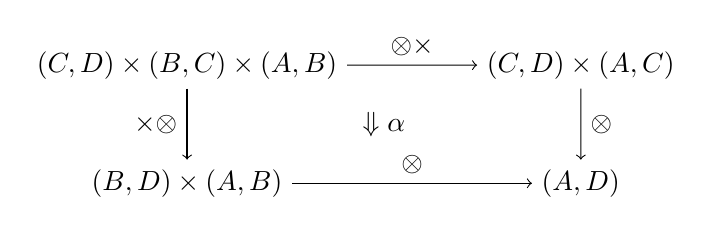
\begin{tikzpicture}[yscale=1.5, xscale=2.5]
\node (A) at (0,1){$\fB(C,D) \times \fB(B, C) \times \fB(A,B)$};
\node (C) at (2,1){$\fB(C,D) \times \fB(A,C)$};
\node (D) at (0,0) {$\fB(B,D)  \times \fB(A,B)$};
\node (E) at (2,0) {$\fB(A, D) $};
\node (B) at (1,.5) {$\Downarrow \alpha$};
\draw[->] (A) to node[above]{$\otimes \times \id$} (C);
\draw[->] (A) to node[left]{$\id \times \otimes$} (D);
\draw[->] (C) to node[right]{$\otimes$} (E);
\draw[->] (D) to node[above]{$\otimes$} (E);
\end{tikzpicture}
\end{document} 

    \end{center}
\item For each two objects $A,B$ of $\fB$, a natural isomorphisms 
  \begin{center}
    %
\documentclass[12pt]{ociamthesis}
\usepackage{tikz}
\newcommand{\id}{\mathrm{id}}
\begin{document}

\begin{equation*}
\begin{aligned}
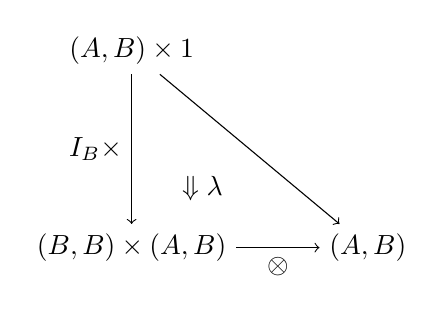
\begin{tikzpicture}[yscale=2.5, xscale=3]
\node (A) at (0,1){$\fB(A,B) \times 1$};
\node (B) at (1,0) {$\fB(A,B)$};
\node (D) at (0,0) {$\fB(B,B) \times \fB(A,B)$};
\node (C) at (.3,.3){$\Downarrow \lambda$};
\draw[->] (A) to node[above]{$\iso$} (B);
\draw[->] (D) to node[below]{$\otimes$} (B);
\draw[->] (A) to node[left]{$  I_B \times \id$} (D);
\end{tikzpicture}
\hspace{1cm}
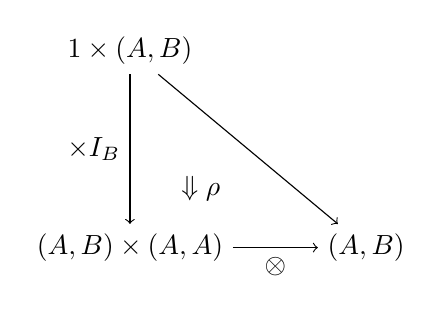
\begin{tikzpicture}[yscale=2.5, xscale=3]
\node (A) at (0,1){$1 \times \fB(A,B)$};
\node (B) at (1,0) {$\fB(A,B)$};
\node (D) at (0,0) {$\fB(A,B) \times \fB(A,A)$};
\node (C) at (.3,.3){$\Downarrow\rho$};
\draw[->] (A) to node[above]{$\iso$} (B);
\draw[->] (D) to node[below]{$\otimes$} (B);
\draw[->] (A) to node[left]{$\id \times I_B$} (D);
\end{tikzpicture}
\end{aligned}
\end{equation*}
\end{document} 

    \end{center}
 \end{itemize}
This data needs to satisfy the usual axioms for bicategories~\cite{maclane}
\end{defn}

The 2-category $\cDbl$ has finite products, which gives the monoidal structure. 
%we can write down the definition of bicategory in terms of hom-categories, with for instance composition functors $\bT(A,B) \times \bT(B,C) \to \bT(A,C)$, and then replace all the hom-categories with hom-double-categories.
%(In other words, we pass through a general notion of bicategory enriched over a cartesian monoidal strict 2-category.)
When we apply the definition above to $\cDbl$, we see that a locally cubical bicategory has objects, hom-double categories {of 1-cells, tight 2-cells, loose 2-cells, and 3-cells which fit in a square of tight and loose 2-cells. We have double functors $\comp$, $I_A$ and tight isomorphisms $\alpha, \rho, \lambda$.

Note that a locally cubical bicategory with one object is precisely a monoidal double category in the sense of \cref{sec:symm-mono-double}, and thus the explicit description of the coherences in \cref{sec:symm-mono-double} can also be applied here.
We will primarily be concerned with the following two examples.

\begin{eg}
  Any category can be regarded as a double category in the \emph{loose} direction, with only identity tight morphisms and identity 2-cells.
  (Note that this is a \emph{strict} double category, not a pseudo one.)
  This operation preserves products, and thereby any strict 2-category can be regarded as a locally cubical bicategory.
  In particular, we will regard the 2-category $\cDblf$ as a locally cubical bicategory in this way; thus it has only identity tight 2-cells and identity 3-cells. We write $\fDblf$ for this locally cubical bicategory.
  % Let $\cDblf$ denote the sub-2-category of $\cDbl$ containing the double categories, all functors between them, and only transformations with loosely strong companions; we regard this as a locally cubical bicategory with only identity \fxnote*{The tight transformations between double categories are the \emph{loose} 2-morphisms in this locally cubical bicategory, right?}{tight} 2-morphisms and identity 3-cells.  The functor $\comp$ is defined on tight transformations as the Godement product. The pseudo double functor $\transid_A: * \rightarrow \cD bl(A,A)$ maps the cells in the trivial double category $*$ to the identity cells and morphisms in $\cD bl(A,A)$. 
\end{eg}

\begin{eg}
  By~\cite[Corollary 12]{gg:ldstr-tricat}, there is a locally cubical bicategory $\fBicat$ defined by the following data:
  \begin{itemize}
  \item Its objects are bicategories.
  \item Its morphisms are functors.
  \item Its loose 2-cells are pseudo natural transformations.
  \item Its tight 2-cells are icons~\cite{lack:icons}.
  \item Its 3-cells are \emph{cubical modifications} as defined in~\cite[Definition 13]{gg:ldstr-tricat}.
  \end{itemize}
\end{eg}

We recall the definition of a cubical modification.

\begin{defn}
Let $F,G,H,K: \cD \rightarrow \cE$ be pseudo functors; let $\alpha: F \Rightarrow G$, $\beta: H \Rightarrow K$ be pseudo transformations; let $\gamma: F \Rightarrow H$, $\delta: G \Rightarrow K$ be icons. A \textbf{cubical modification}
\[
\begin{tikzpicture}
\node (tl) at (0,1) {$F$};
\node (tr) at (1,1) {$G$};
\node (bl) at (0,0) {$H$};
\node (br) at (1,0) {$K$};
\draw[doubletight] (tl) to node[above]{$\alpha$} (tr);
\draw[doubletight] (bl) to node[below]{$\beta$} (br);
\draw[doubletight] (tl) to node[left]{$\gamma$} (bl);
\draw[doubletight] (tr) to node[right]{$\delta$} (br);
\node at (.5,.5) {$\DDownarrow \Gamma$};
\end{tikzpicture}
\]
is given by a family of 2-cells $\Gamma_A: \alpha_A \RRightarrow \beta_A$ such that for every 1-cell $f:A \rightarrow B$ of $\cD$, the following equality holds.

 \begin{equation}
 \begin{aligned}
 \begin{tikzpicture}[scale=1.5]
 \node (tl) at (-1,1) {$FA$};
 \node (tm) at (0,1) {$FB$};
 \node (tr) at (1,1) {$GB$};
 \node (bl) at (-1,0) {$FA$};
 \node (bm) at (0,0) {$GA$};
 \node (br) at (01,0) {$GB$};
 \node (bl1) at (-1,-.7){$HA$};  
 \node (bm1) at (0,-.7) {$KA$};
 \node (br1) at (1,-.7) {$KB$}; 
 \draw[doubletight] (tm)  to node[above]{$\alpha_B$} (tr);
 \draw[doubleeq] (bm) to (bm1);
 \draw[doubletight] (bm) to node[above] {$Gf$}(br);
 \draw[doubleeq] (tr) to (br);
 \draw[doubleeq] (tl)  to  (tm);
 \draw[doubleeq] (tl) to (bl);
 \draw[doubletight] (tl) to node[above]{$Ff$}(tm);
 \draw[doubletight] (bl) to node[above]{$\alpha_A$}(bm);
 \node at (0,.5) {\footnotesize $\Downarrow \alpha_f$}; 
 \node at (0.5,-.3) {\footnotesize $\Downarrow \delta_f$}; 
  \node at (-0.5,-.3) {\footnotesize $\Downarrow \Gamma_A$};
 \draw[doubletight] (bl1)  to node[above]{$\beta_A$} (bm1);
 \draw[doubletight] (bm1) to  node[above]{$Kf$}(br1);
 \draw[doubleeq] (bl)  to (bl1);
 \draw[doubleeq] (br)  to (br1);
 \end{tikzpicture}
 \end{aligned}
 =
\begin{aligned}
 \begin{tikzpicture}[scale=1.5]
 \node (tl) at (-1,1) {$FA$};
 \node (tm) at (0,1) {$FB$};
 \node (tr) at (1,1) {$GB$};
 \node (bl) at (-1,0) {$HA$};
 \node (bm) at (0,0) {$HB$};
 \node (br) at (01,0) {$KB$};
 \node (bl1) at (-1,-.7){$HA$};  
 \node (bm1) at (0,-.7) {$KA$};
 \node (br1) at (1,-.7) {$KB$}; 
 \draw[doubletight] (tm)  to node[above]{$\alpha_B$} (tr);
 \draw[doubleeq] (tm) to (bm);
 \draw[doubletight] (bm) to node[above] {$\beta_B$}(br);
 \draw[doubleeq] (tr) to (br);
 \draw[doubleeq] (tl)  to  (tm);
 \draw[doubleeq] (tl) to (bl);
 \draw[doubletight] (tl) to node[above]{$Ff$}(tm);
 \draw[doubletight] (bl) to node[above]{$Hf$}(bm);
 \node at (-0.5,.5) {\footnotesize $\Downarrow \gamma_f$}; 
 \node at (0.5,.5) {\footnotesize $\Downarrow \Gamma_B$}; 
 \draw[doubletight] (bl1)  to node[above]{$\beta_A$} (bm1);
 \draw[doubletight] (bm1) to  node[above]{$Kf$}(br1);
 \draw[doubleeq] (bl)  to (bl1);
 \draw[doubleeq] (br)  to (br1);
 \node at (0,-0.3) {\footnotesize $\DDownarrow \beta_f$}; 
 \end{tikzpicture}
 \end{aligned}
\end{equation}

\end{defn}

The double functor $\transid_A: * \rightarrow \fBicat(A,A)$ maps the cells in the trivial bicategory $*$ to the identity cells and morphisms of $\fBicat(A,A)$. 
The double functor $\comp$ is defined on functors of bicategories by composition. On pseudo transformations and icons it is given by the Godement product. On cubical modifications it is defined below:

\begin{equation*}
\begin{aligned}
 \begin{tikzpicture}[scale=2]
 \node (tl) at (-1,1) {$FF'A$};
 \node (tm) at (0,1) {$GF'A$};
 \node (tr) at (1,1) {$GG'A$};
 \node (bl) at (-1,0) {$HF'A$};
 \node (bm) at (0,0) {$KF'A$};
 \node (br) at (01,0) {$KG'A$};
 \node (bl1) at (-1,-1){$HH'A$};  
 \node (bm1) at (0,-1) {$KH'A$};
 \node (br1) at (1,-1) {$KK'A$}; 
 \draw[doubletight] (tm)  to node[above]{$G(\alpha'_A)$} (tr);
 \draw[doubleeq] (tm) to (bm);
 \draw[doubletight] (bm) to node[above] {$K(\alpha'_A)$}(br);
 \draw[doubleeq] (tr) to (br);
 \draw[doubleeq] (tl)  to  (tm);
 \draw[doubleeq] (tl) to (bl);
  \draw[doubleeq] (bm) to (bm1);
 \draw[doubletight] (tl) to node[above]{$\alpha_{F'A}$}(tm);
 \draw[doubletight] (bl) to node[above]{$\beta_{F'A}$}(bm);
 \node at (-0.5,.5) {\footnotesize $\Downarrow \Gamma_{F'A}$}; 
 \node at (0.5,.5) {\footnotesize $\Downarrow \delta_{\alpha'_A}$}; 
 \draw[doubletight] (bl1)  to node[above]{$\beta_{H'A}$} (bm1);
 \draw[doubletight] (bm1) to  node[above]{$K(\beta'A)$}(br1);
 \draw[doubleeq] (bl)  to (bl1);
 \draw[doubleeq] (br)  to (br1);
 \node at (-.5,-0.5) {\footnotesize $=$}; 
\node at (.5,-0.5) {\footnotesize $\DDownarrow K\Gamma'_A$}; 
\end{tikzpicture}
\end{aligned}
\end{equation*}
%%%%%%%%%

Functoriality follows from naturality of the icons. Note that there are several equivalent ways to define this composition on cubical modifications, by choosing different versions of the Godement product.  

Now, we can similarly obtain the notion of \emph{functor} between locally cubical bicategories from the definition of a $\mathcal{V}$-enriched functor between $\mathcal{V}$-enriched bicategories.

\begin{defn}\label{def:lcbcfunc}
Let $\mathcal{V}$ be a monoidal 2-category. Let ${\fB,\fC}$ be $\mathcal{V}$-enriched bicategories. A $\mathcal{V}$-enriched functor $F: {\fB} \rightarrow {\fC}$ consists of the following data:
\begin{enumerate}
\item An assignment on objects that sends each object $A$ of ${\fB}$ to an object $F A$ of ${\fC}$.
\item For each two objects $A,B$ of ${\fB}$, a 1-cell ${\fB}(A,B) \rightarrow {\fC}(F(A),F(B))$ of $\mathcal{V}$.
\item For every triple of objects $A,B,C$ of ${\fB}$, a 2-cell of $\mathcal{V}$ 
\begin{align} 
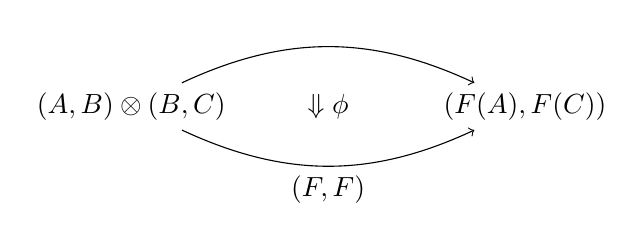
\begin{tikzpicture}
\node(1) at (0,0) {${\fB}(A,B) \otimes {\fB}(B,C)$};
\node(2) at (5,0) {${\fC}(F(A),F(C))$};
\draw[->] (1) to[in=155, out=25] node[above]{$\fB \comp $} (2); 
\draw[->] (1) to[in=-155, out=-25] node[below]{$ \comp (F,F)$} (2); 
\node at (2.5,0) {$\Downarrow \phi \iso$};
\end{tikzpicture}
\end{align}
\item For every object $A$ of ${\fB}$ a 2-cell of $\mathcal{V}$
\begin{align}
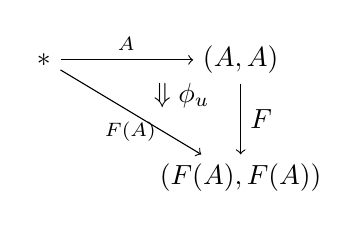
\begin{tikzpicture}[xscale=.5, yscale=.3]
\node(1) at (0,0) {$*$};
\node(2) at (5,0) {${\fC}(A,A)$};
\node(3) at (5,-5) {${\fB}(F(A),F(A))$};
\draw[->] (1) to node[above]{$\looseid_{A}$} (2); 
\draw[->] (1) to node[below]{$\looseid_{F(A)}$} (3);
\draw[->] (2) to node[right]{$F$} (3); 
\node at (3.5,-1.5) {$\Downarrow \phi_u \iso$};
\end{tikzpicture}
\end{align}
\item The usual coherence diagrams, Definition 10 of~\cite{nick:tricatsbook} commute.
\end{enumerate}
\end{defn}

When we apply this definition to the monoidal 2-category $\cDbl$, we see that a {\bf functor of locally cubical bicategories} $F$ consists of a map of objects $A \mapsto F A$; pseudo double functors ${\fB}(A,B) \rightarrow {\fC}(F(A),F(B))$ for each two objects $A,B$; and tight transformations $\phi$ for each two objects $A,B$ of ${\fB}$, and $\phi_u$ for every object $A$ of ${\fB}$, plus axioms.

\begin{thm}\label{thm:h-functor}
The map $\cL$ gives rise to a functor of locally cubical bicategories $\cL \maps \fDblf\to \fBicat$.
\end{thm}
\begin{proof}
Note that the 1-functor $\cH:\mathbf{Dbl}\to\mathbf{Bicat}$ has a left adjoint that regards a bicategory as a double category with only identity tight 1-cells.
Thus, the functor of bicategories $\cDblf(\D,\E) \rightarrow \cBicat(\cH(\D), \cH (\E)) = \cH( \fBicat(\cH(\D),\cH(\E)))$ has an adjunct pseudo double functor $\fDblf(\D,\E) \rightarrow \fBicat(\cH\D, \cH \E)$. Consequently, the first two requirements in \autoref{def:lcbcfunc} are satisfied by Theorems \ref{thm:1-func} and \ref{thm:h-locfr}.
Since $\cH$ strictly preserves composition of 1-cells,
the third requirement amounts to the existence of a tight transformation $\phi\maps \behat * \alhat \iso \widehat{\be*\al}$ for every pair of transformations with loosely strong companions 

  \[\vcenter{\xymatrix{\lC \rtwocell^F_G{\al} & \lD \rtwocell^H_K{\be}
      & \lE}}\]
      
      such that 
%
 \begin{equation}
        \vcenter{\xymatrix@-.5pc{
        1_{{\cH}H \odot {\cH}F} \ar[r]\ar[d]_{=} &
        \hat{1}_{H}* \hat{1}_{F}\ar[d]^{\phi}\\
        1_{{\cH}(H \odot F)}\ar[r] &
        \widehat{1_{H} * 1_{F}}}} \quad\text{and}\quad       
    \vcenter{\xymatrix@-.5pc{
        \widehat{\gm\al}* \widehat{\de\be} \ar[r]\ar[d]_\phi &
        (\gmhat* \dehat)\circ(\alhat* \behat)\ar[d]^{\phi * \phi}\\
        \widehat{\gm\al* \de\be}\ar[r] &
        (\widehat{\gm* \de})\circ(\widehat{\al* \be})}}
  \end{equation}
commute. 
Here, we use the 'Godement product' $*$ of 2-cells in $\cDbl$.  

  Now by Lemmas \ref{thm:comp-compose} and
  \ref{thm:comp-func}, $(\behat *\alhat)_A = \behat_{GA} \circ
  H(\alhat_A)$ is a companion of $(\be*\al)_A = \be_{GA} \circ
  H(\al_A)$.  Therefore, we take the component $(\phi_{\alpha,\beta})_A$ to be
  \[\theta_{\behat_{GA} \circ H(\alhat_A),\, \widehat{\be*\al}_A}.\]
 As the other morphisms in the diagrams above are also $\theta$-isomorphisms, the equations hold by Lemma~\ref{thm:theta-compose-vert}.
For the tight transformation  $\phi_u$ we can simply take the identity, since $\cH$ is strictly unital.
The coherence equations hold by Lemma~\ref{thm:theta-compose-vert}
\end{proof}


Our goal is to enhance this functor to act on ``monoidal objects''.
It is well-known that ``monoidal functors preserve monoid objects'', so our approach will be to categorify this: we will show that the functor $\cH$ is monoidal, in an appropriate sense, and that monoidal functors of this sort preserve monoidal objects of the appropriate sort.

In fact, the monoidality of $\cH$ is easy to describe, because the monoidal structures of $\fDblf$ and $\fBicat$ are cartesian and very strict.

In general, if $\mathcal{V}$ is a monoidal 2-category with strict 2-categorical finite products (such as \cDbl), we say that a $\mathcal{V}$-enriched bicategory ${\fB}$ has \textbf{finite products} when for each two objects $C,D \in {\fB}$ there is an object $C\times D$ with projections $C\times D\to C$ and $C\times D\to D$ (i.e.\ morphisms $I\to \fB(C\times D,C)$ and $I\to \fB(C\times D,D)$ in \cV) inducing an \emph{isomorphism} in $\mathcal{V}$ (not merely an equivalence):
%
\begin{align}
\fB(A, C \times D) \xrightarrow{\cong} \fB(A,C) \times \fB(A,D)
\end{align}
and similarly there is a strict terminal object $\ast$ such that $\fB(A,\ast)$ is strictly terminal in \cV\ for all $A$.
This holds for \fBicat\ and \fDblf, because cartesian products of bicategories and double categories are simply componentwise, and all the morphisms in \fBicat\ and \fDblf\ (no matter how weak) are defined in terms of data in their targets.

Similarly, we say that a functor $F$ of \cV-enriched bicategories \textbf{preserves products} if it takes the terminal object to a terminal object and pairs of product projections $A \leftarrow A\times B \to B$ to pairs of product projections (in the above strict sense).

\begin{thm}
The functor of locally cubical bicategories $\cH: \fDblf \rightarrow \fBicat$ preserves products.
\end{thm}
\begin{proof}
Since $\cH$ merely forgets a part of the double categories and double functors, we have simple equalities
$\cH(\mathbb{D} \times \mathbb{E}) = \cH(\mathbb{D}) \times \cH(\mathbb{E})$, and the product projections are likewise preserved.
The case of the terminal object is likewise easy.
\end{proof}

% Local Variables:
% TeX-master: "smbicat"
% End:
